\documentclass[12pt,a4paper]{jbook}
\usepackage{mm-thesis}
\usepackage[dvipdfmx]{graphicx}
\usepackage{cite}
\usepackage{comment}
\usepackage{docmute}
\usepackage{color}
%\usepackage{amsmath}
%\usepackage{amsthm}
%\usepackage{amsfonts}

\begin{document}
\newpage

\chapter{事例研究}
本章では、複数の具体的な事例を取り上げ、提案モデルの実装の正しさを確認する。

\section{キャッシュの基本動作}
本節では、提案モデルでのキャッシュの実装の正しさを確認する。
提案モデルにおいて、キャッシュは主に格納、再利用、検証の三つの動作を行う。
それぞれについて、実行ツールAlloy Analyzerの実行結果を確認する。

\subsection{レスポンスの格納}
レスポンスの格納動作を確認するため、実行結果からレスポンスの格納を伴う動作を抽出する。
ここでは簡単のため、最も単純な二者間における通信で生じるレスポンスの格納を対象とし、Code\ref{code:test_store}を用いて出力を得る。
Code\ref{code:test_store}はクライアントとサーバの二者間における一組のリクエストとレスポンスの通信において、格納レスポンス集合に要素が存在するキャッシュの状態が存在する結果を出力するものである。

\begin{lstlisting}[caption=レスポンスの格納, label=code:test_store]
run test_store{
	#HTTPClient = 1
	#HTTPServer = 1
	#HTTPRequest = 1
	#HTTPResponse = 1
	some CacheState.dif.store
} for 2
\end{lstlisting}

得られる出力結果を整理し、図\ref{fig:TestStore}に示す。
図\ref{fig:TestStore}には、PrivateCache0を持つBrowser0とServer0間の、Request0とResponse0のトランザクションにおけるキャッシュの状態変化が示されている。
最初、リクエスト時にはキャッシュの状態はCacheState0で示されており、CacheState0の変化要素を表すCacheDifItem0のstoreが空集合である。
しかし、レスポンス時には状態はCacheState1に変化しており、対応するCacheDifItem1がResponse0にstoreを指している。
以上より、図\ref{fig:TestStore}はあるトランザクションにおいて、レスポンスがブラウザキャッシュに格納されている状態を表しており、レスポンスの格納が表現可能であることが確認できる。

\begin{figure}[htb]
\centering
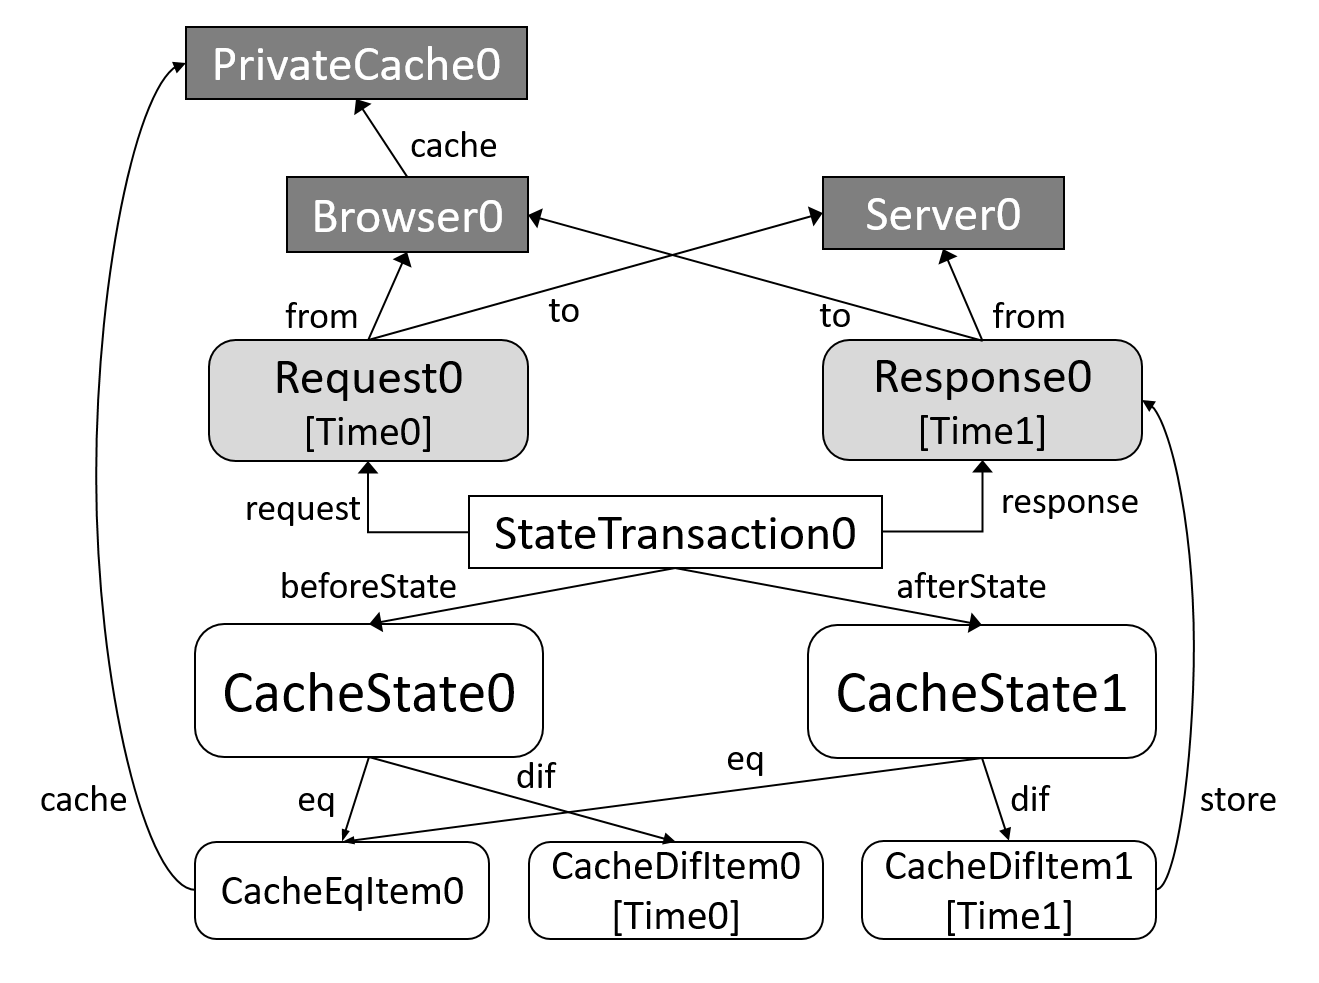
\includegraphics[width=450pt]{./fig/TestStore.eps}
\caption{レスポンスを格納する状態の一例}
\label{fig:TestStore}
\end{figure}

\subsection{格納レスポンスの再利用}
レスポンスの再利用動作を確認するため、実行結果からレスポンスの再利用を伴う動作を抽出する。
ここでは簡単のため、最も単純な二者間における通信で生じるレスポンスの再利用を対象とし、Code\ref{code:test_reuse}を用いて出力を得る。
Code\ref{code:test_reuse}はクライアントとサーバの二者間における二組の通信において、一度レスポンスの再利用が発生している結果を出力するものである。

\begin{lstlisting}[caption=格納レスポンスの再利用, label=code:test_reuse]
run test_reuse{
	#HTTPClient = 1
	#HTTPServer = 1
	#Cache = 1

	#HTTPRequest = 2
	#HTTPResponse = 1
	#CacheReuse = 1
} for 4
\end{lstlisting}

得られる出力結果をスペースの都合上一部簡略化し、図\ref{fig:TestReuse}に示す。
図\ref{fig:TestReuse}はあるキャッシュを持つブラウザとサーバ間で、同様のURIに対してリクエストが二回送信された状態を表している。
ここで、StateTransaction0では図\ref{fig:TestStore}と同様、ブラウザキャッシュにResponse0を格納している。
StateTransaction1では、この格納レスポンスを再利用するイベントCacheReuse0が発生している。
以上より、図\ref{fig:TestReuse}に示す出力結果から、再利用を伴う動作が表現可能であることが確認できる。

\begin{figure}[htb]
\centering
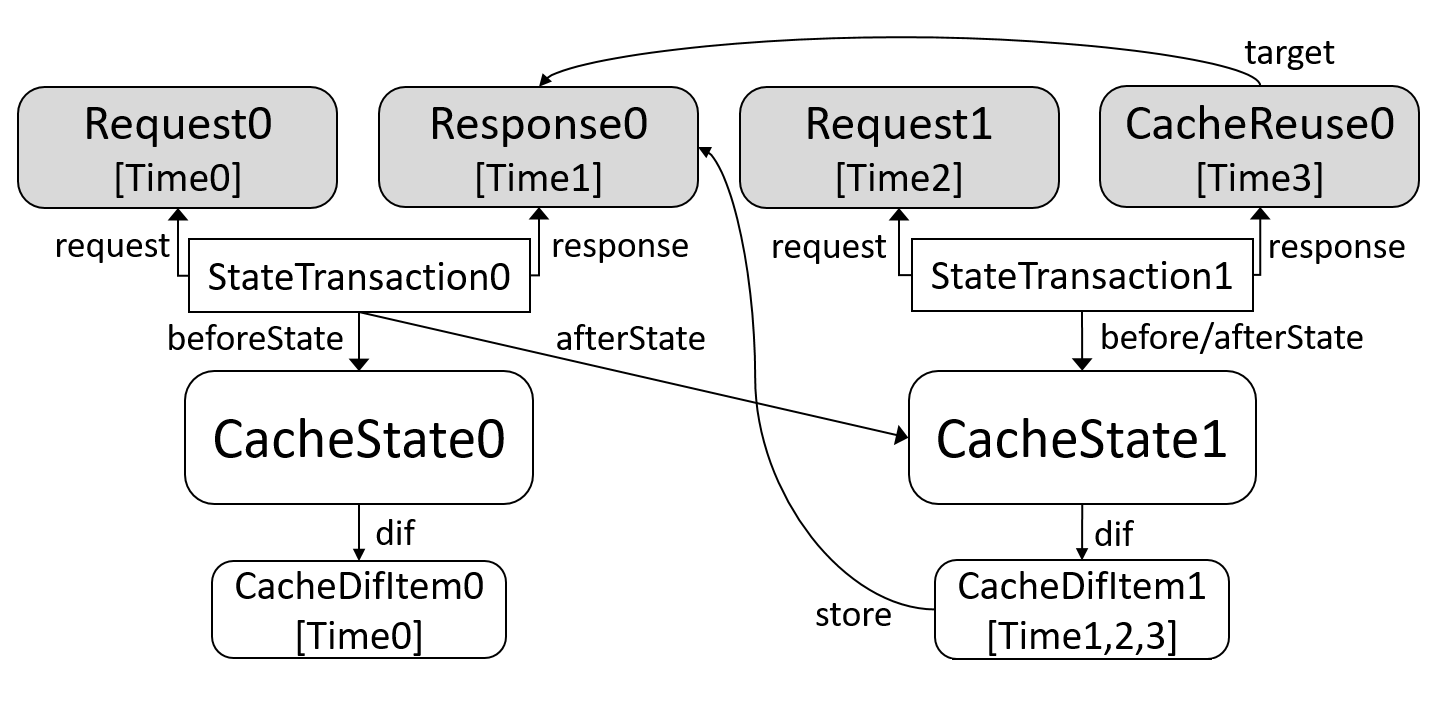
\includegraphics[width=450pt]{./fig/TestReuse.eps}
\caption{格納レスポンスを再利用する状態の一例}
\label{fig:TestReuse}
\end{figure}

\subsection{格納レスポンスの検証}
レスポンスの検証動作を確認するため、実行結果からレスポンスの検証を伴う動作を抽出する。
ここでは簡単のため、最も単純な二者間における通信で生じるレスポンスの検証を対象とし、Code\ref{code:test_verification}を用いて出力を得る。
Code\ref{code:test_verification}はクライアントとサーバの二者間における三組の通信のうち、検証が行われた通信が存在する結果を出力する。
ここで検証が行われたかの判定は、\ref{sec:CacheVerification}節で述べたCode\ref{code:checkVerification}を利用している。

\begin{lstlisting}[caption=格納レスポンスの検証, label=code:test_verification]
run test_verification{
	#HTTPClient = 1
	#HTTPServer = 1
	#HTTPIntermediary = 0
	#Cache = 1
	#PrivateCache = 1

	some str:StateTransaction | checkVerification[str]
} for 6
\end{lstlisting}

得られる出力結果をスペースの都合上一部簡略化し、図\ref{fig:TestVerification}に示す。
図\ref{fig:TestVerification}はあるキャッシュを持つブラウザとサーバ間での、三つの通信(StateTransaction0,1,2)が存在している状態を表しており、このうちStateTransaction2が検証を行っている通信である。
まず、StateTransaction0では図\ref{fig:TestStore}と同様、ブラウザキャッシュにResponse0を格納している。
次に、Request2に対してブラウザキャッシュ内に格納されているResponse0を再利用するため、StateTransaction2で検証動作を行っている。
ここで、格納レスポンスのResponse0にはEtagHeaderが含まれているため、検証に用いる条件付きリクエストであるRequest1にはIfNoneMatchHeaderが含まれている。
また、検証結果となるResponse1は再利用可能であることを示す304の状態コードとなっているため、Response0はそのまま再利用可能であることが示されている。
以上を踏まえて、StateTransaction1ではResponse0をそのまま再利用している。

\begin{figure}[htb]
\centering
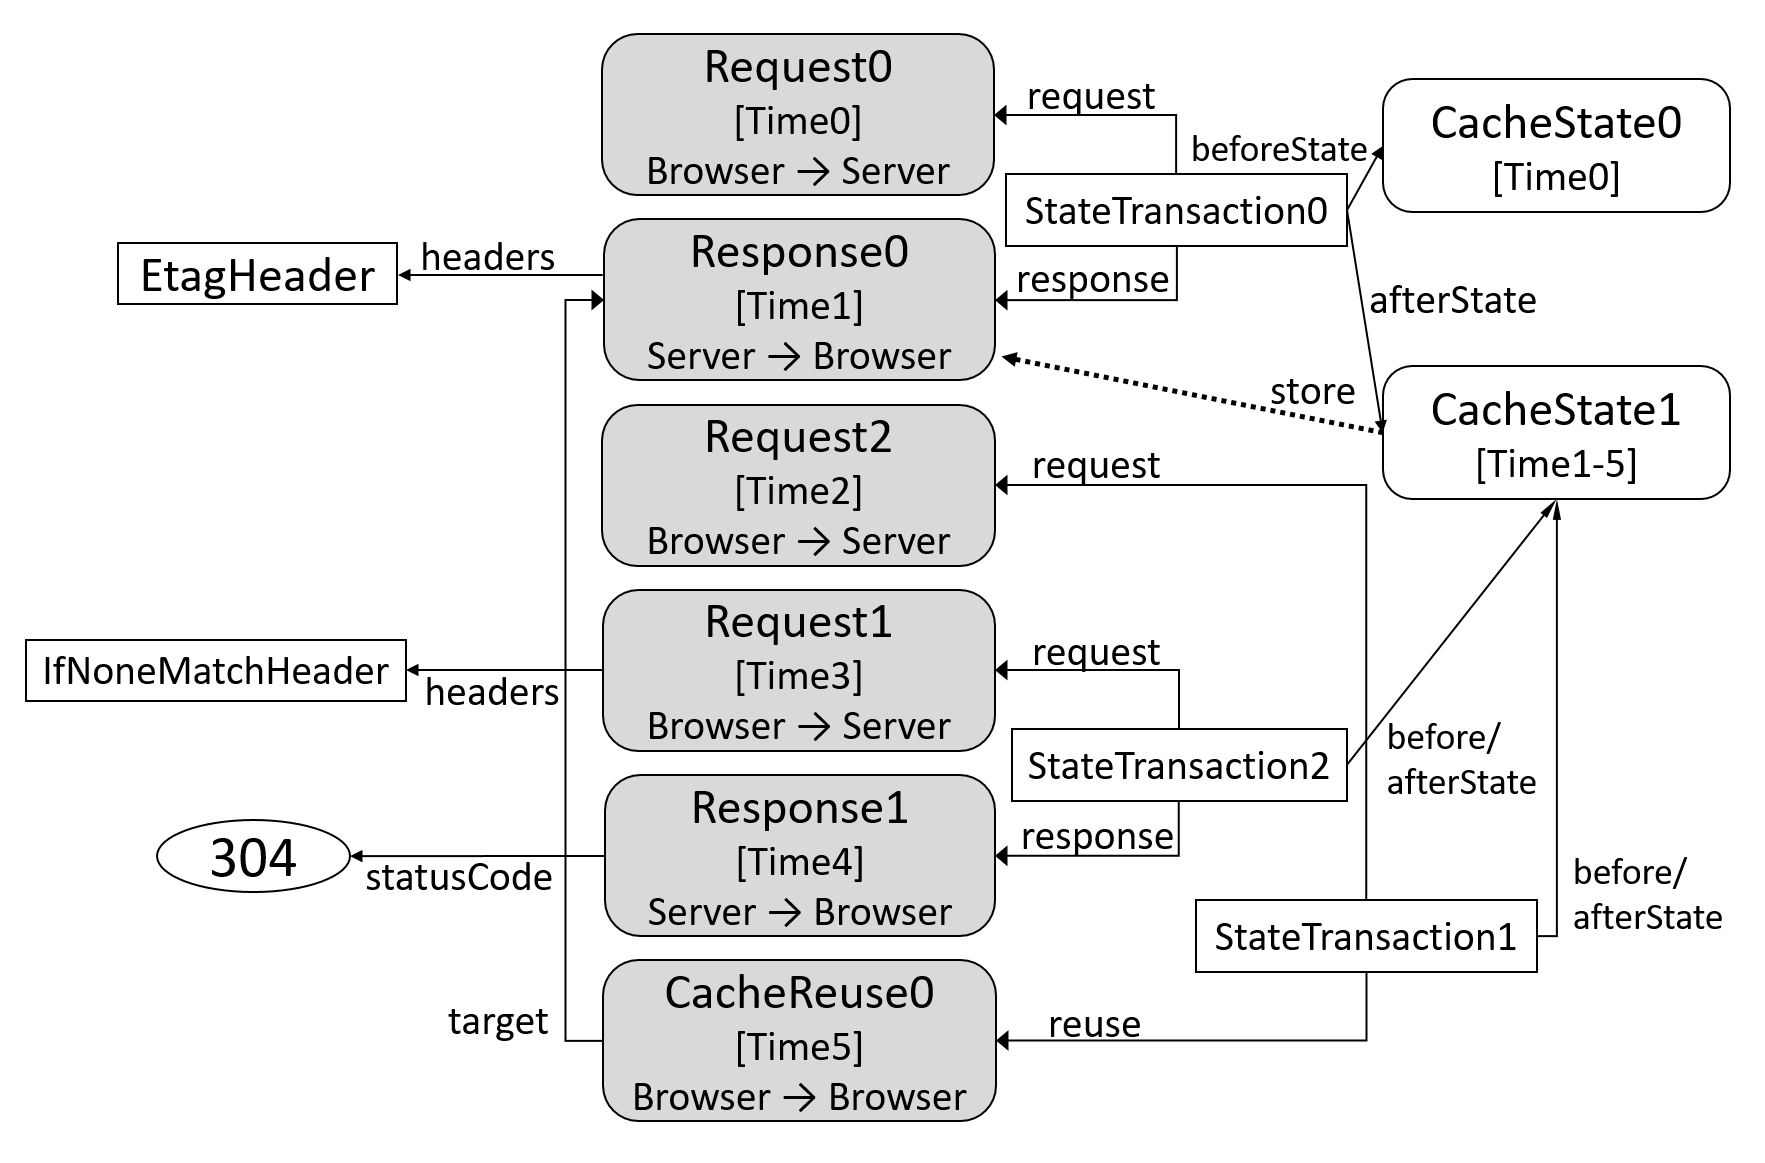
\includegraphics[width=450pt]{./fig/TestVerification.eps}
\caption{格納レスポンスの検証が含まれる状態の一例}
\label{fig:TestVerification}
\end{figure}

\section{中継者の基本動作}

\section{Same-origin Browser Cache Poisoning Attack}
提案モデルでSame-origin Browser Cache Poisoning Attack\cite{bcpattack}が表現可能であるかを確認する。

\subsection{攻撃シナリオ}


\section{Cross-origin Browser Cache Poisoning Attack}
\subsection{攻撃シナリオ}


\section{Web Cache Deception Attack}
\subsection{攻撃シナリオ}


\section{Cross-site Request Forgeries Attack}
\subsection{攻撃シナリオ}


\end{document}
